\section{User Study 2}

We want to realize what's a good gyro control. 

\begin{enumerate}
\item Range of gyro movement\\
ask them directly.
\item The precision of gyro(relavent target size?)\\
observe data.
\end{enumerate}

\subsection{Result expectation}

\begin{figure}[!t]
\centering
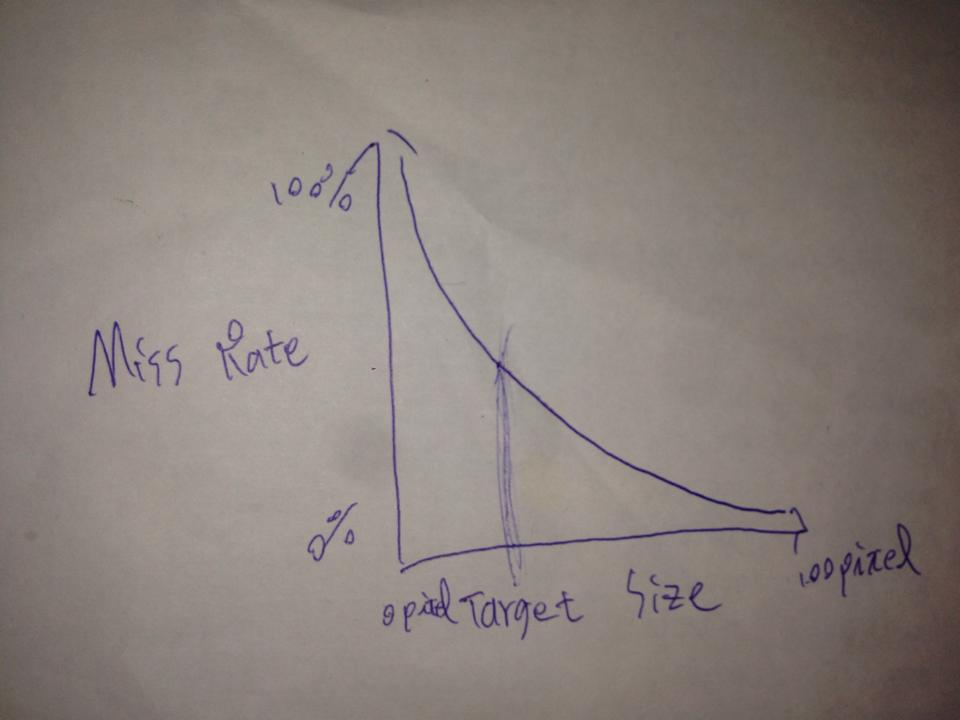
\includegraphics[width=0.9\columnwidth]{Figures/US2_missRate.jpg}
\caption{Hi I'm Small Sun.}
\label{fig:PS_Frus}
\end{figure}

\begin{figure}[!t]
\centering
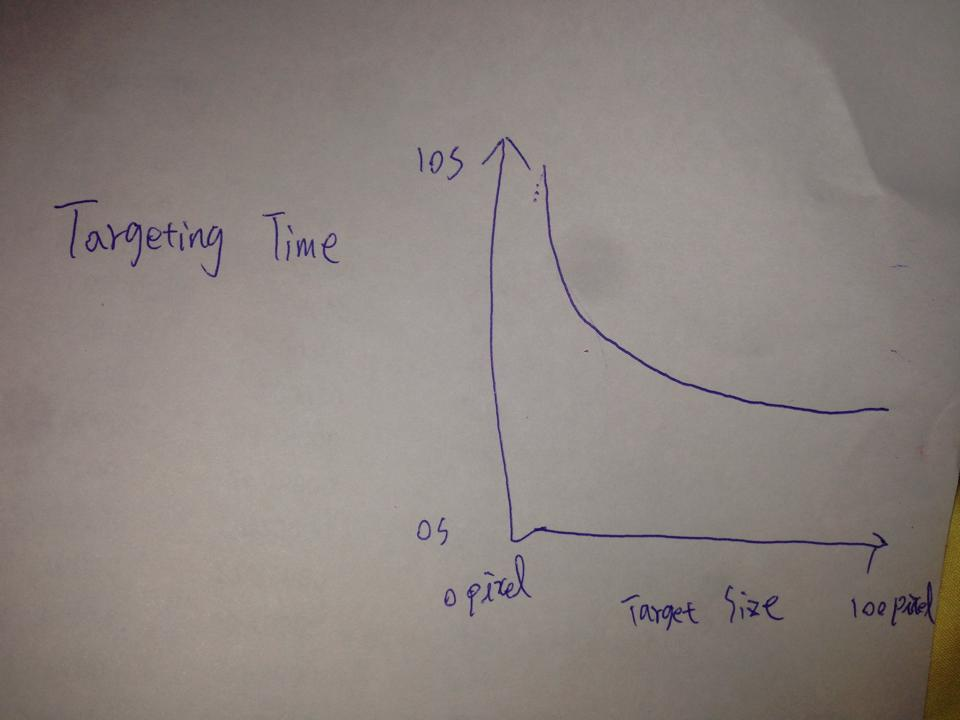
\includegraphics[width=0.9\columnwidth]{Figures/US2_targetingTime.jpg}
\caption{Hi I'm Small Sun.}
\label{fig:PS_Frus}
\end{figure}

\begin{figure}[!t]
\centering
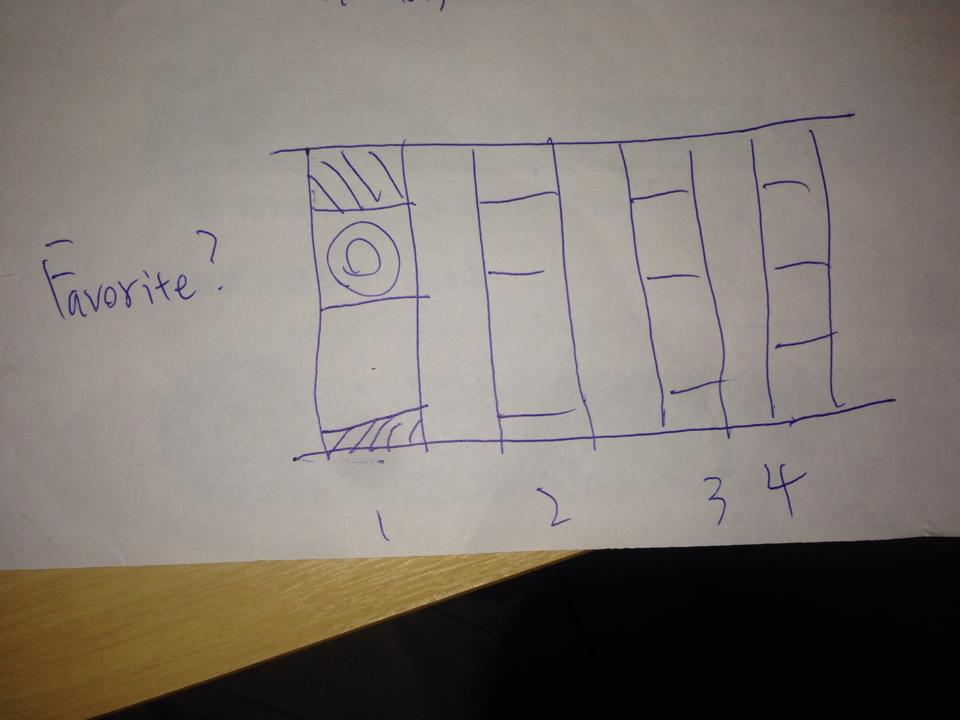
\includegraphics[width=0.9\columnwidth]{Figures/US2_favoriteFire.jpg}
\caption{Hi I'm Small Sun.}
\label{fig:PS_Frus}
\end{figure}

\begin{figure}[!t]
\centering
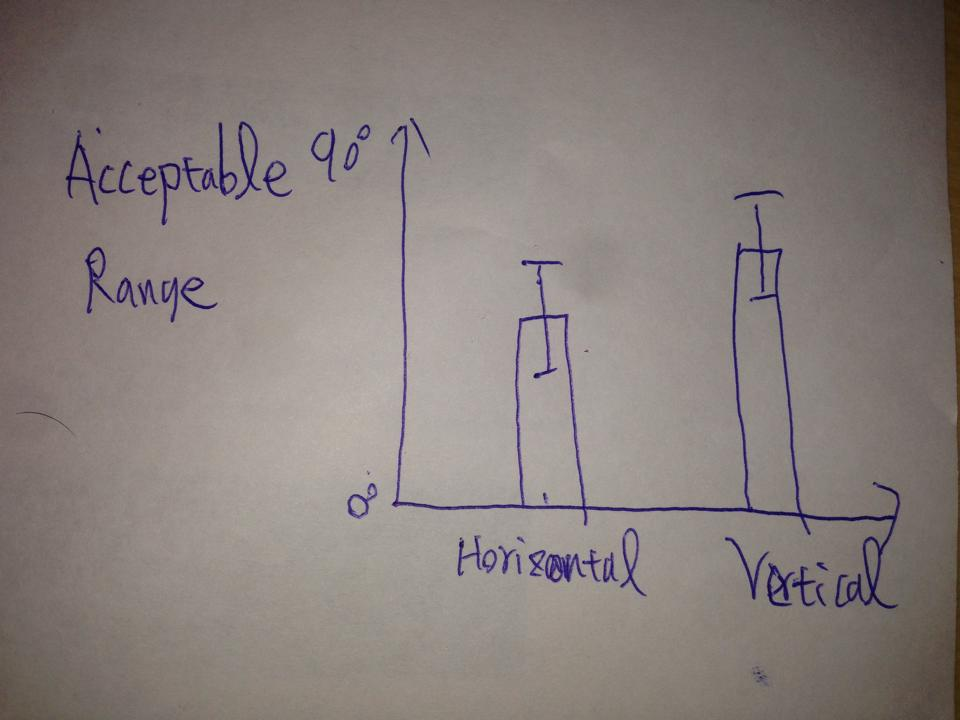
\includegraphics[width=0.9\columnwidth]{Figures/US2_acceptableRange.jpg}
\caption{Hi I'm Small Sun.}
\label{fig:PS_Frus}
\end{figure}

\begin{figure}[!t]
\centering
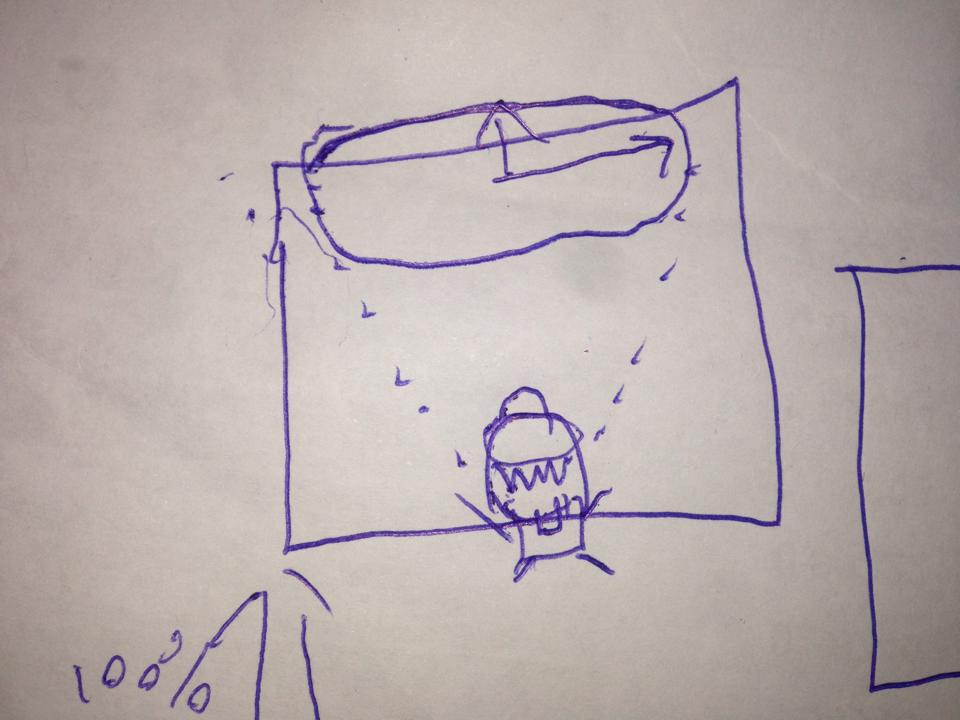
\includegraphics[width=0.9\columnwidth]{Figures/coverPhoto2.jpg}
\caption{Hi I'm Small Sun.}
\label{fig:PS_Frus}
\end{figure}


fire
\begin{enumerate}
\item Use mobile phone
\item Tapping google glass's touch pad
\item Voice control
\item Eye blinking
\end{enumerate}

